%% Local IspellDict: brasileiro

\documentclass[11pt]{article}
\usepackage{relatorio-pibic}
\usepackage[utf8x]{inputenc}
\usepackage{cite}
\usepackage{subfig}
\usepackage{rotating}

% usar para palavras estrangeiras: \eng{english word}
\newcommand{\eng}[1]{\textit{#1}}

\begin{document}

\graphicspath{{figs/}}

\cabecalho{Relatório Final}

\dadosRelatorioFinal
{Levantamento de operações de teorias de contornos em análises de
  obras musicais}
{Verificando inconsistências nas teorias de contornos musicais através
  de ferramentas computacionais }
{Eduardo Lago Nunes}
{Marcos da Silva Sampaio}
{Genos}
{Teoria de Relações de Contornos Musicais, Teoria Musical, Computação Musical}
{JANEIRO A JULHO DE 2012}

\resumo{Inserir texto do resumo}

\newpage

\setcounter{page}{1}
\onehalfspace

\Section{Introdução}
\label{sec:introducao}
\info{Delimitação do problema trabalhado e as conexões entre o plano
  de trabalho do bolsista e o projeto do orientador. Objetivos e
  justificativa do plano em termos de relevância para a pesquisa
  cientifica e do estado da arte.}
% importância de contornos para música, da teoria de contornos, a
% inconsistência...

Contorno é uma linha que marca externamente uma figura ou um objeto,
uma espécie de perímetro, caminho que cerca o redor de algum lugar ou
algo. Em música pode-se visualizar o contorno de diversos aspectos
como altura, densidade, ritmo, timbre, etc.
\cite[p. 01]{Sampaio2008}.
% Marcos: Use sempre o número da figura ou tabela para fazer a
% referência. NUNCA use figura/tabela/exemplo seguinte. Corrigi o
% problema neste local e mudei a forma de escrita. Siga o exemplo onde
% houver o mesmo problema.
% Marcos: fale em poucas palavras o que são os números
As figuras~\ref{fig:melodia} e \ref{fig:30142} contêm uma melodia e a
representação gráfica de seu contorno.

\begin{figure}[h]
  \centering
  \subfloat[Melodia]{
    \includegraphics{melodia}
    \label{fig:melodia}
  }
  \subfloat[Contorno < 3 0 1 4 2 >]{
    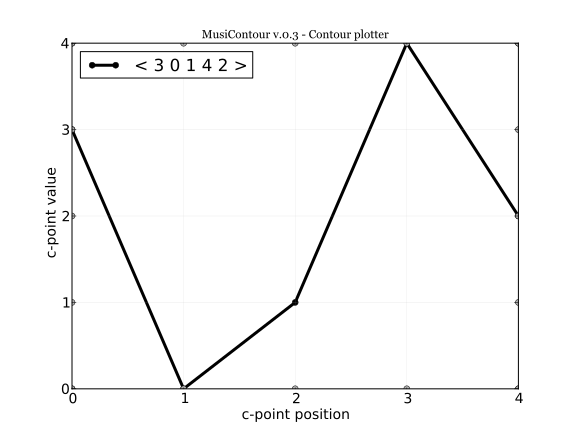
\includegraphics[scale=.3]{30142}
    \label{fig:30142}
  }
  \caption{Melodia e representação do contorno de alturas}
  \label{fig:melodia-representacao}
\end{figure}

% Marcos: Clifford: aspecto estrutural em webern
% Marcos: ver análises de obras com enfoque nos contornos
% Marcos: usar altura no lugar de notas
Contornos são importantes por serem mais perceptíveis que alturas
até mesmo para ouvintes destreinados.
\cite[p. 225]{Marvin1987}.

Diversos autores desenvolveram a Teoria de Relações de Contornos
Musicais \cite{Friedmann1985, Friedmann1987, Morris1987, Marvin1987,
  Marvin1988, Polansky1992, Morris1993, Clifford1995, Quinn1997,
  Beard2003, Sampaio2008, Schultz2008, Schultz2009, Bor2009}. Esta
teoria dispõe de ferramentas que ajudam a entender os contornos.
% Marcos: "O orientador deste trabalho..."
% Eduardo: Ok
O orientador deste trabalho vem desenvolvendo programas computacionais para
auxiliar no cálculo de contornos musicais.
% Marcos: Eu desenvolvi apenas um software, no singular. Não diga que
% foi encontrada a inconsistência. Não use a voz passiva. Use voz
% ativa e dê o crédito: "Ele identificou a inconsistência do
% algoritmo..."
% Eduardo: Ok
Durante o desenvolvilmeto do software ele identificou a
inconsistência do algoritmo de forma prima de Marvin e Laprade
\cite{Marvin1987}. Esta inconsistência pode implicar em fragilidades
nas ramificações desta teoria.
% Marcos: fica melhor se você disser: "Dessa forma foi necessário
% verificar o impacto..."
% Eduardo: Ok
Dessa forma foi necessário verificar o
impacto dela nas referências bibliográficas.
% Marcos: 'desenvolvi e alimentei'
Para economizar tempo e energia na busca por operações de contornos,
tive como trabalho criar um mapa de operações para consultas rápidas.
Neste mapa estão contidas 508 operações que foram
encontradas nas referências bibliográficas.

% nas seções seguintes descrever as coisas
\Section{Materiais e métodos}
\label{sec:materiais}
\info{Descrição da maneira como foram desenvolvidas as atividades para
  se chegar aos objetivos propostos. Indicar o material e métodos que
  foram usados.}

Para o desenvolvimento do mapeamento de operações usamos os seguintes
materias.

\begin{enumerate}
\item Mapa de operações de contornos. Vide mais
  informações na seção resultados.
% Marcos: remover 'este programa'
\item Mendeley\footnote{Disponível em
    \url{http://www.mendeley.com/}}. Repositório colaborativo dos
  textos da pesquisa. Este programa foi necessário para o
  compartilhamento da bibliografia.
\item MusiContour\footnote{Disponível em
    \url{http://genosmus.com/MusiContour}.}. Software de processamento
  de operações de contornos desenvolvido pelo orientador. Esta
  ferramenta foi necessária para realizar os testes de operações de
  contornos.
\item Python\footnote{Disponível em
    \url{http://www.python.org/getit/}.}. Linguagem de programação
  utilizada para desenvolvimento do MusiContour. A operação do
  MusiContour requer conhecimentos básicos desta linguagem.
% Marcos: falar do linux e do ubuntu, como falei em outra nota
\item Linux\footnote{Disponível em
  \url{http://www.ubuntu.com/download/desktop}.}. Sistema operacional
  de código aberto onde o MusiContour foi testado integralmente e
  tem instalação mais simples.
\item Git\footnote{Disponível em
    \url{http://git-scm.com/downloads}.}. Sistema de controle de
  versão distribuído com ênfase em velocidade. Ferramenta utilizada
  para organização do projeto e para controle de versão do relatório
  final.
\item Github\footnote{Disponível em
    \url{https://github.com/}.}. Repositório central de projetos com
  controle de versão Git.
% Marcos: inverter ordem
  Além das tarefas diárias\footnote{As tarefas realizadas estão
    disponíveis para consulta em \url{http://goo.gl/4Ie7c}.}, usamos o
  github para mater a versão de desenvolvimento do MusiContour.
% Marcos: falar como um texto
\item \LaTeX{} e Kile\footnote{Disponível em
  \url{http://kile.sourceforge.net/}.}. \LaTeX: sistema completo de tipografia
  de textos acadêmicos. Kile: editor da sintaxe do \LaTeX.
\end{enumerate}

Para realização do trabalho foram cumpridas as seguintes etapas.

\begin{enumerate}
\item Familiarização com o objeto da pesquisa de 01/01/2012 à 30/01/2012.
Consistiu na leitura da literatura sobre contornos, produção de resenhas
e sessões de dúvidas com o orientador.
\item Alimentação da planilha de operações, de 23/01/2012 à 06/06/2012.
Mapeamento de todas as operações contidas nas referência
bibliográficas.
\item Treinamento com ferramentas Linux/Ubuntu, Python e MusiContour, de 20/06/2012 à 11/07/2012.
Ferramentas utilizadas para auxiliarem no trabalho.
\item Revisão das operações mapeadas, de 28/06/2012 à 04/07/2012.
Revisão dos cálculos de todas as operações que foram mapeadas na planilha.
\end{enumerate}

% Marcos: explicar como fez o mapeamento
O mapeamento de operações iniciado pelo bolsista anterior precisava
ser revisado e formatado.  Procurei operações de contornos
relacionadas a obras da literatura musical e adicionei ao mapa de
operações.
% Marcos: remover parágrafo abaixo. mandar leitor ver resultados e
% tabela com planilha
A planilha tem o recurso classificação, elas estão organizadas em
referência, operação, página, obra, compositor, gráfico.  Este recurso
é útil para buscar as operações diretamente.

% Marcos: Use primeira pessoa: "Após a alimentação com os dados sobre
% operações de contornos, testei manualmente..."
Cada operação do mapa de operações foi testada tanto manualmente para os
cálculos mais simples, quanto utilizando o MusiContour para os cálculos mais
complexos. Para utilizar o MusiContour foi necessário um treinamento em Python,
em MusiContour e também a instalação do sistema operacional
Linux/Ubuntu.
% Marcos: O único programa necessário foi o MusiContour. Então não
% fale "dos programas necessários". Você pode falar "MusiContour e
% suas dependências".
Utilizei o Linux/Ubuntu para
agilizar a instalação e utilização dos proramas necessários. O MusiCountour não
havia sido testado no windows, sistema que eu usava, e não
tinhamos tempo para testá-lo, então optamos por utilizar o
Linux/Ubuntu.
% Marcos: melhor "Esta escolha foi bem sucedida..."
% Eduardo: Ok
Esta escolha foi bem sucedida, pois apreder a utilizar o software
% Marcos: "foi mais prático"
% Eduardo: Ok
foi mais prático.

% Marcos: dizer que ele formata o texto automaticamente
Finalmente para elaborar o relatório utilizei o \LaTeX, que permite
uma facilidade no trabalho de edição, um aprendizado adicional sobre
programação, e um aprofundamento nos materiais.

\Section{Resultados}
\label{sec:resultados}
\info{Relação dos resultados ou produtos obtidos durante a execução da
  pesquisa, indicando os avanços no conhecimento disponível obtidos
  com a execução da pesquisa.}

% planilha com mapeamento de operações e o que funciona
% aprendizado

O principal resultado deste trabalho é o mapa das operações de
contornos musicais presentes nas referências bibliográficas sobre este
tema. Este mapa contém 508 operações encontradas nas referências
bibliográficas. A tabela~\ref{tab:mapa-operacoes} contém um fragmento
deste mapa. Ele funciona como um catálogo de operações, utilizado para
consultas rápidas de uma determinada operação de contorno (vide seção
de discussão).

\begin{sidewaystable}
  \centering
  \begin{tabular}{r|lllllll}
    Referência: Autor, ano e título&Operação&Página&Composição&Compositor&Exemplo&Demonstração&Teste\\
    \hline
    Friedmann85:methodology&ccvi&235&Pierrot Lunaire, Die Blasse Waescherin&Schoenberg&7&gráfico&OK\\
    Friedmann85:methodology&ccvi&236&Pierrot Lunaire, Die Blasse Waescherin&Schoenberg&1º Parágrafo&texto&OK\\
    Friedmann85:methodology&ccvii&235&Pierrot Lunaire, Die Blasse Waescherin&Schoenberg&7&gráfico&OK\\
    Friedmann85:methodology&ccvii&236&Pierrot Lunaire, Die Blasse Waescherin&Schoenberg&2º parágrafo&texto&OK\\
    Friedmann85:methodology&ccvii&240&Phantasy op. 47&Schoenberg&3º parágrafo&texto&Erro? 0, 2, 1, 3, 5, 4\\
    Friedmann85:methodology&ccvii&241&Phantasy op. 47&Schoenberg&8.a, 8.b&gráfico&Erro? 0, 2, 1, 3, 5, 4\\
    Friedmann85:methodology&cia&231&Phantasy, op. 47&Schoenberg&1º parágrafo&texto&OK\\
    Friedmann85:methodology&cia&235&Pierrot Lunaire, Die Blasse Waescherin&Schoenberg&7&gráfico&OK\\
    Friedmann85:methodology&cia&236&Pierrot Lunaire, Die Blasse Waescherin&Schoenberg&2º parágrafo&texto&OK\\
    Friedmann85:methodology&cis&231&Suite, op. 25, Menuett&Schoenberg&3º parágrafo&texto&OK\\
    Friedmann85:methodology&cis&233&Phantasy op. 47&Schoenberg&6&gráfico&OK\\
    Friedmann85:methodology&inversion&225&five piano pieces, op. 23, Waltz&Schoenberg&1.a, 1.b&gráfico&OK\\
    Friedmann85:methodology&inversion&226&five piano pieces, op. 23, Waltz&Schoenberg&4º parágrafo&texto&OK\\
    Friedmann85:methodology&inversion&229&Phantasy op. 47&Schoenberg&4&gráfico&OK\\
    Friedmann85:methodology&inversion&231&Suite, op. 25, Menuett&Schoenberg&3º parágrafo&texto&OK\\
    Friedmann85:methodology&rotation&225&Phantasy op. 47&Schoenberg&2&gráfico&OK\\
    Friedmann85:methodology&rotation&226&Phantasy op. 47&Schoenberg&3º parágrafo&texto&OK\\
    Friedmann85:methodology&rotation&233&Phantasy, op. 47&Schoenberg&4a, 4b&gráfico&OK\\
    Friedmann85:methodology&rotation&231&Phantasy op. 47&Schoenberg&5º parágrafo&texto&OK\\
  \end{tabular}
  \caption{Fragmento do mapa de operações de contornos}
  \label{tab:mapa-operacoes}
\end{sidewaystable}

Além do mapa de operações, este trabalho teve como resultados os
testes destas operações e as inconsistências encontradas nestes testes
(vide lista abaixo). Estas inconsistências terão análises posteriores,
pois a verificação de seu impacto na teoria requer tempo.

\begin{enumerate}
\item \eng{Contour Class Vector II} \cite[p. 241]{Friedmann1985}.
\item \eng{Contour Similarity} \cite[p. 242]{Quinn1997}.
\item \eng{Contour Similarity} \cite[p. 262]{Quinn1997}.
\item \eng{Contour Class} \cite[p. 113]{Schultz2008}.
\end{enumerate}

Este trabalho teve ainda os seguintes resultados secundários:

\begin{enumerate}
\item Aprofundamento do conhecimento sobre contornos.
% Marcos: o mais importante no início sempre. qual dessas ferramentas
% você só poderia aprender nesta pesquisa?
% Eduardo: A ordem seria essa?
\item Aprendizado sobre Linux/Ubuntu, Python, Kile, MusiContour.
\item Aprimoramento da escrita de textos acadêmicos.
\item Aprimoramento da leitura em língua inglesa.
\item Aprimoramento de organização e técnicas de estudo.
\end{enumerate}

\Section{Discussão}
\label{sec:discussao}
\info{Expor de modo sucinto a contribuição do seu projeto ao projeto
  de pesquisa do orientador e ao conhecimento científico da sua área,
  apresentando as implicações para futuros trabalhos que podem ser
  desenvolvidos.}
% comentar o que foi dito nas outras seções. ir além da descrição

O mapa de operações tem como sua principal função agilizar a procura por
algum tipo operação que esteja contida em alguma das referências bibliográficas.
% Marcos: mostrar na tabela
Este mapa está subdividido em: Artigo, tipo de operação, página, obra, compositor,
texto ou gráfico, parágrafo ou figura. Embora nas referências bibliográficas existam
mais de 508 operações, no mapa estão datados apenas as operações que foram retiradas
de exemplos musicais.

% Marcos: O mais importante primeiro. Fale do MusiContour antes do
% github.
% Eduardo: Ok
Utilizei os materiais citados para dar mais agilidade no trabalho e para
economizar tempo e enrgia.
% Marcos: "Por exemplo, o MusiContour realiza cálculos..."
% Marcos: exemplos de uso: calcular redução de contornos, comparação
% difusa contornos
Como o MusiContour por exemplo, fazer cálculos extensos pode ser algo
demorado, principalmente calcular uma matriz. Além do trabalho de
calcular uma matriz é muito mais demorado calcular a similaridade
entre duas matrizes, isso sem contar que durante os cáculos podemos
confundir algum número ou sinal e gerar um trabalho muito maior. O
MusiContour resolve tudo com a agilidade de uma calculadora
economizando tempo e energia.

Por exemplo, a tabela~\ref{tab:matriz-comparacao-contornos} contém a
matriz de comparação do contorno < 3 0 1 4 2 >
(fig.~\ref{fig:melodia-representacao}). Para calcularmos a matriz
devemos comparar todos os números do contorno entre si, para isso
posicionamos os números do contorno em forma de linha e coluna.
% Marcos: mastigue para o leitor: "A primeira linha contém a
% comparação do elemento 3 com o próprio elemento 3 (0), em seguida
% com o elemento 0 (-) e assim por diante..."
% Eduardo: Ok
A primeira linha contém a comparação do elemento 3 com o próprio elemento 3 (0),
em seguida com o elemento 0 (-) e assim por diante. Se os números forem iguais,
sua comparação terá valor zero. Se o valor da linha for menor que o valor da
coluna adicionamos o sinal de subtração. Se o valor da linha for maior
que o valor da conluna adicionamos o sinal de Adição.

\begin{table}
  \centering
  \begin{tabular}{c|ccccc}
    &3&0&1&4&2\\
    \hline
    3&0&-&-&+&-\\
    0&+&0&+&+&+\\
    1&+&-&0&+&+\\
    4&-&-&-&0&-\\
    2&+&-&-&+&0\\
  \end{tabular}
  \caption{Matriz de comparação de contornos}
  \label{tab:matriz-comparacao-contornos}
\end{table}

% Marcos: "O Github ajuda...."
% Marcos: ajudou também na hora de citar os períodos de trabalho no
% relatório
Outro software utilizado para ganharmos tempo foi o Github, é possível definir os
prazos das tarefas e categorizá-las de acordo com a necessidade do trabalho.

% Marcos: "Por exemplo, a tabela~\ref{tab:matriz-comparacao-contornos}
% contém a matriz de comparação do contorno < 3 0 1 4 2 >
% (fig.~\ref{fig:melodia-representacao})". Use a notação correta de
% contornos.
% Eduardo: Ok

% Marcos: que substituição você fez? figuras para banco de dados e
% tutorial online por testes de operações.
% Marcos. substituir treinamento por 'familiarização'. ver em metodologia
Entrei como bolsista substituto em 02/01/2012. Isso resultou na
necessidade de um treinamento que consumiu doi meses e onze dias.
% Marcos: você tem o tempo exato do treinamento. Basta olhar os emails
% e o github. Ser preciso nessas coisas mostra organização para quem
% lê. Você pode incluir o tempo que levamos tentando instalar o
% MusiContour no Windows
Faltando cerca de um mês para terminamos a pesquisa, fizemos um
remanejamento no plano de trabalho devido este tempo que o treinamento
consumiu. Este remanejamento foi o teste das operações contidas no
mapeamento.

% Marcos: repetir o objetivo do projeto
O teste das operações é importante porque está diretamente
relacionado ao objetivo principal do projeto.
% Marcos: mover para o final
Com esses testes pude também aprimorar meus conhecimentos no uso dos
softwares MusiContour e python.

A pesquisa me possibilitou um contato direto com as referência
bibliográficas que abordavam o tema contornos.  A teoria de contornos
não está no conteúdo programático do curso de graduação em composição.
A partir do trabalho como bolsista pude estudar profundamente esta
teoria.  Além disso me ajudou a aprimorar a leitura da lígua inglesa,
escrita e conscisão de resenhas, e um conhecimento sobre diversas
ferramentas computacionais.

%%%%%%%%% bibliografia %%%%%%%%%%%%%%%%
% insere bibliografia

\renewcommand{\refname}{Referências bibliográficas (máximo 15)}
\info{Relação itemizada das referências que subsidiam a proposta de
  pesquisa, colocando as mais importantes.}

\nocite{
  Friedmann1985,
  Friedmann1987,
  Morris1987,
  Marvin1987,
  Marvin1988,
  Polansky1992,
  Morris1993,
  Clifford1995,
  Quinn1997,
  Beard2003,
  Sampaio2008,
  Schultz2008,
  Schultz2009,
  Bor2009
}

\bibliographystyle{plain}
\bibliography{bibliography}

\Section{Participação em reuniões científicas e publicações}
\info{Relacionar as reuniões científicas e os títulos dos trabalhos
apresentados pelo estudante durante a vigência da bolsa. Incluir
títulos de publicações que resultaram ou se beneficiaram de seu
trabalho.}

\Section{Anexos}
\info{Anexar os resumos ou trabalhos que foram apresentados pelo bolsista
durante a vigência da bolsa.}

\end{document}
